
\begin{figure}[ht!]
    \centering
    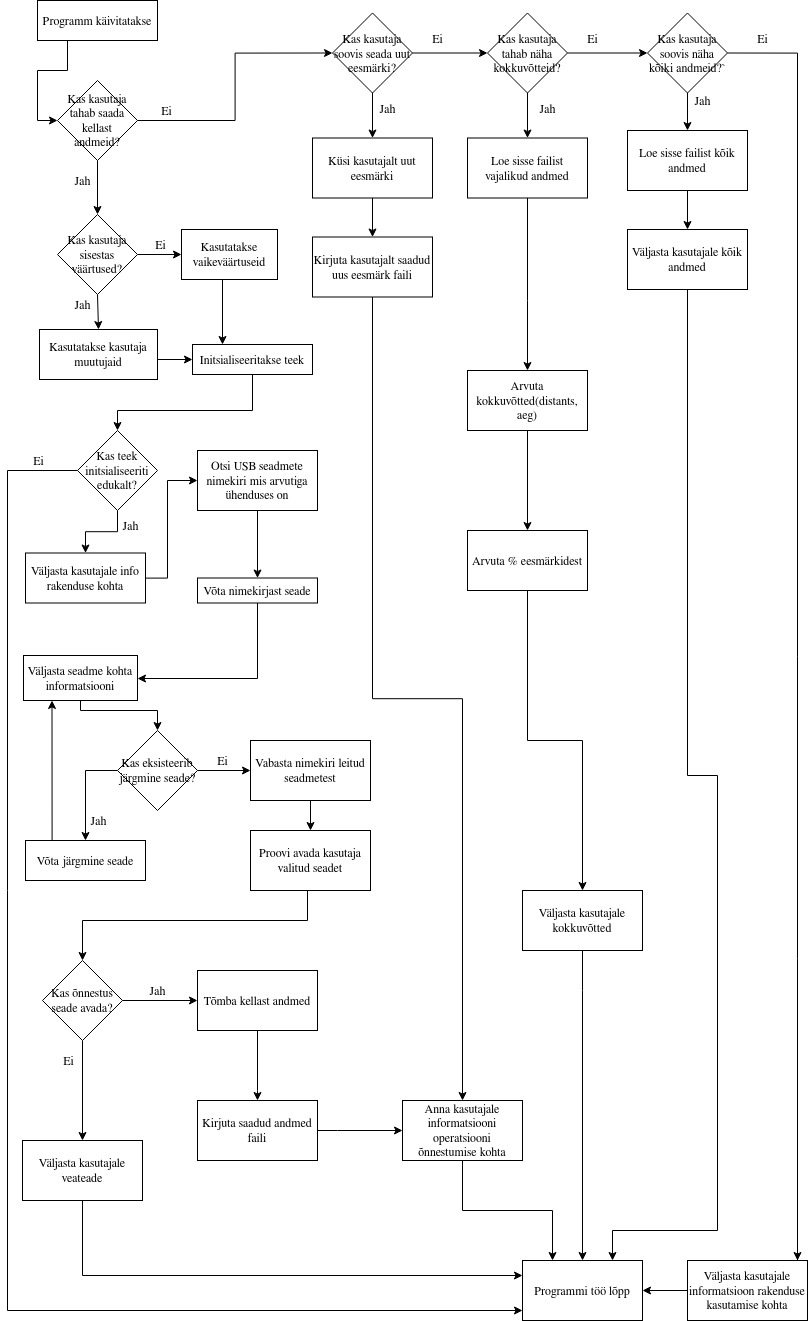
\includegraphics[width=.75\textwidth]{figures/flowchart.jpg}
    \caption{\textit{Voodiagramm programmi planeeritud tööst}}
    \label{fig:flowchart}
\end{figure}
\pagebreak

\section{Olemasoleva programmi töö}\label{sec:programmi-too}
Programmi alguses määratakse ära vaikeväärtused, mida rakendus saab kasutada.
Seejärel initsialiseeritakse \textit{libusb} teek ning antakse kasutajale teada mis versioon teegist kasutusel on.
Kui kasutaja on andnud rakendusele kaasa parameetrid, mille järgi soovib leida seadet, millega suhelda siis otsitakse seda konkreetset seadet ja kui kasutaja ei ole neid kaasa andnud, kastuatakse vaikeväärtuseid.
Kui otsitavat seadet ei leita, lõpetatakse programmi töö.
Kui otsitav seade on olemas ja ligipääsetav, siis programm jätkab seadme kohta informatsiooni väljastamisega.
Enne kellale päringute saatmist peab seadme avama, mida ka tehakse.
Kui avamine õnnestub, teatakse kasutajale, et see õnnestus, kui ei siis programmi töö katkestatakse.
Seejärel peaks hakkama kellast informatsiooni hankimine, kuid seda programmi osa projekti raames valmis ei saadud.

\section{Programmi fookus}\label{sec:arenduskaik}
Vaadates joonist~\ref{fig:flowchart} on näha, et kõige detailsemalt on kirjeldatud andmete hankimise osa ning rakenduse kasutajapoolne osa on lihtsam.
Rakenduse arenduse käigus otsustati, et proovitakse saada andmete saamise osa enne valmis, kui hakatakse kasutaja poolt valmistama.
Sellise valiku tingis võimalikkus 3 lõpptulemuse vahel.

Esimene neist oleks programm, mis suudab tõmmata kellast andmed ja on muus osas poolik.
Selline lahendus oli parim saavutatav tulemus, kuna sinna otsa kasutajaliides ehitada oleks olnud kiirem protsess ja see oli ühtlasi ka antud programmi kontekstis vähemtähtis.
Teine variant oleks olnud alustada kasutajaliidesega ja suunata see käsitsi kirjutatud faili lugema ja sealt andmeid võtma. 
Seda ei valitud kuna lõppeesmärgi saavutamiseks, mis oli siis kellast saadud andmete töötlemine, oleks pidanud topelt tööd tegema, kuna käsitsi kirjutatud fail poleks ilmselt olnud ühilduv kellast tulnud andmetega.  
Esimesega kaasaskäiv kõige halvem võimalik tulemus oli, et projekti lõpuks ei valmi ei andmete hankimise osa, kui ka kasutajaliides, nii et projekt jääb ilma töötava programmita.

Eelnevalt loetletud lõpptulemuste vahel valides vaadati, milline osa projektist kõige tähtsam on.
Kasutaja andmete analüüsimise koha pealt oleks tulnud just esimesena teha valmis kasutajaliides.
Projekti suurim eesmärk aga oli luua liides just Polar kellale, millega oleks kasutajatel ligipääs enda kogutud andmetele, millega siis edasi toimida.
Loetletud põhjused tingisidki vajaduse saada esimesena andmed kätte ja õigustasid riski projekt mitte valmis saada.